\section{Алгоритм решения задачи и численные примеры}\label{sec:experiments}
Представим алгоритм решения задачи управления.
В соответствии с~\eqref{eq:model} градиент функционала качества равен
\[
    J'_\lambda (u) = \lambda u - p_2.
\]
Здесь $u\in U$ -- управление в граничном условии~\eqref{eq:boundary-2}, $p_2$ -- соответствующая компонента
сопряженного состояния из системы~\eqref{eq:model}--\eqref{eq:model}.

Предлагаемый алгоритм решения задачи (CP) выглядит следующим образом:
%\begin{algorithm}[H]
%    \caption{Алгоритм градиентного спуска}
%    \begin{algorithmic}[1]
%        \State Выбираем значение градиентного шага $\varepsilon$,
%        \State Выбираем количество итераций $N$,
%        \State Выбираем начальное приближение для управления $u_0 \in U$,
%        \For{$k \gets 0,1,2,\dots,N$}
%            :
%            \State Для данного $u_k$ рассчитываем состояние $y_k = \{\theta_k, \varphi_k\}$ --
%            решение задачи~\eqref{eq1},\eqref{bc1}.
%            \State Рассчитываем значение функционала качества $J_\lambda(\theta_k, u_k)$.
%            \State Рассчитываем сопряженное состояние $p_k=\{p_{1k},p_{2k}\}$ из уравнений~\eqref{OC1},
%            где $ \hat{\theta} := \theta_k, \hat{u}=u_k$.
%            \State Пересчитываем управление $u_{k+1} = u_k - \varepsilon (\lambda u_k - p_2)$
%        \EndFor
%    \end{algorithmic}
%\end{algorithm}
Значение параметра $\varepsilon$ выбирается эмпирически таким образом, чтобы значение
$\varepsilon (\lambda u_k - p_2)$ являлось существенной поправкой для $u_{k+1}$.
Количество итераций $N$ выбирается достаточным для выполнения условия
$J_\lambda(\theta_k, u_k) - J_\lambda(\theta_{k+1}, u_{k+1}) < \delta$, где $\delta>0$ определяет точность расчетов.

Примеры, рассмотренные ниже, иллюстрируют работоспособность предложенного алгоритма при
малых значениях параметра регуляризации $\lambda \leq 10^{-12}$.
В первом примере выполнены тестовые расчеты для куба.

Отметим, что для численного решения прямой задачи с заданным
управлением использовалась слабая формулировка
и метод Ньютона для линеаризации задачи.
Решение сопряженной системы, которая является линейной при
заданной температуре, не вызывает трудностей.
Для численного моделирования использовался солвер FEniCS~\cite{fenics, dolfin}.

\textbf{Пример 1.}
Приведем примеры расчетов для куба
$\Omega = {(x, y, z), 0 \leq x,y,z \leq l}$.
Будем считать, что $l=1~\text{см}$, $a = 0.006[\text{см}^2/\text{c}]$,
$b=0.025[\text{см}/\text{с}]$,
$\kappa_a=1[\text{см}^{-1}]$, $\alpha = 0.(3)[\text{см}]$.
Указанные параметры соответствуют стеклу~\cite{Grenkin5}.
Параметр регуляризации $\lambda=10^{-12}.$

Пусть граничные данные имеют следующий вид:
\begin{gather*}
    \theta_n = 0.5 \quad
    \theta_b = 0.1 + z/2 \quad
    \psi_0 = 0.
\end{gather*}
Применяя алгоритм градиентного спуска
с начальным приближением $u_0 = 0.1$, находим приближенное решение
$\{\theta_\lambda,\varphi_\lambda,u_\lambda\}$ задачи (CP)\@.
Для демонстрации того, что алгоритм находит приближенное решение задачи с данными
Коши для температуры, важно сравнить значения $\partial_n\theta_\lambda$ на $\Gamma$ с $q_b.$

На рисунке~\ref{fig1:img_test_1} представлены изолинии модуля относительной разности
$|\partial_n\theta_\lambda-\theta_n|/\ \theta_n$
на грани куба в плоскости $z=l$, где
$\partial_n\theta_\lambda=\partial\theta_\lambda/\partial z$,
а также динамика функционала качества, определяющего
норму разности $\|\theta_\lambda -\theta_b\|^2_\Gamma$.
На остальных гранях куба значения имеют тот же порядок малости.

\begin{figure}[H]
    \centering
    \subfloat[$|\partial_n \theta_\lambda - \theta_n|/\ \theta_n$]
    {
        \label{fig1:img_test_1}
        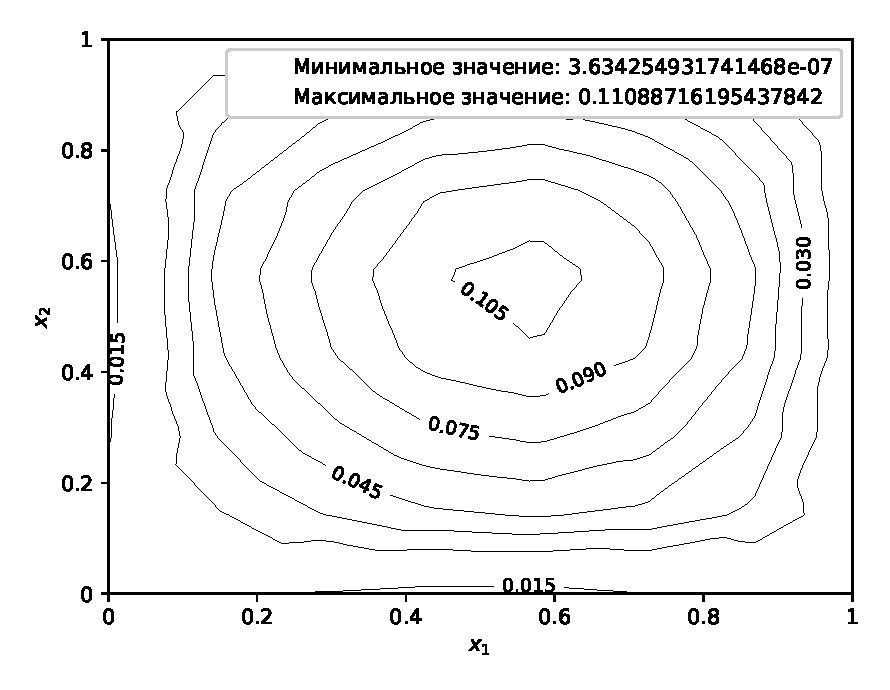
\includegraphics[width=.49\linewidth]{img/exp1_iso}
    }
    \subfloat[Изменение функционала в зависимости от числа итераций]
    {
        \label{fig1:quality}
        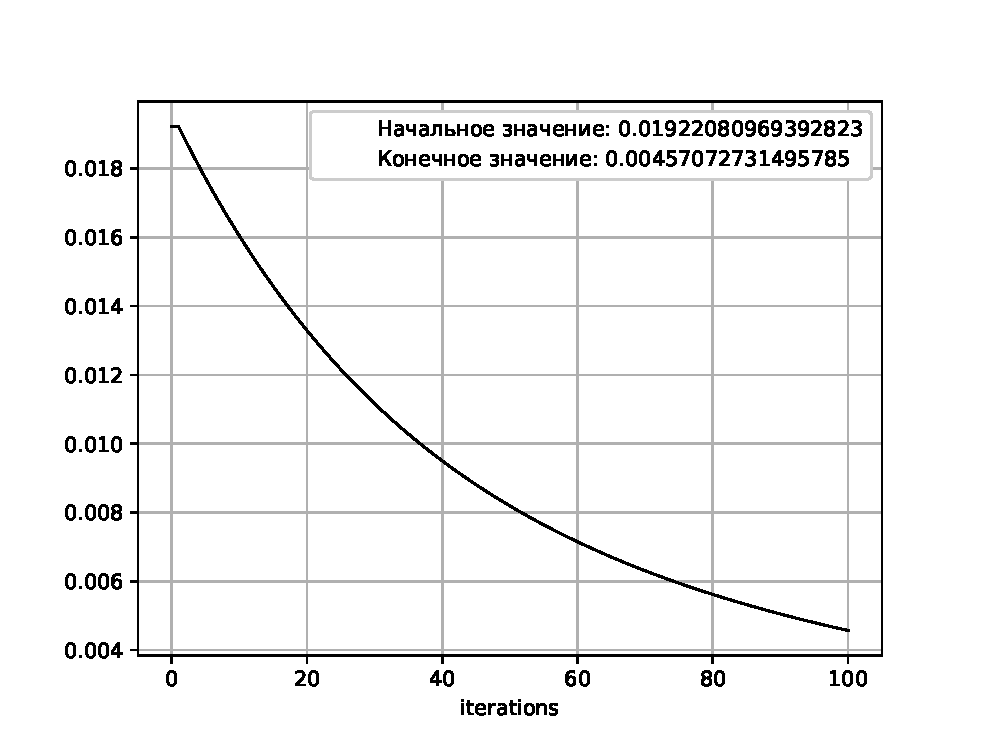
\includegraphics[width=.49\linewidth]{img/exp1_quality}
    }
    \caption{Результаты первого эксперимента}
    \label{fig1}
\end{figure}
